\documentclass[12pt,t]{beamer}
\usetheme{Warsaw}
\usepackage[utf8]{inputenc}
\usepackage[english]{babel}
\usepackage{amsmath}
\usepackage{amsfonts}
\usepackage{amssymb}
\usepackage{graphicx}
\author{Jaskeerat Singh Saluja (2019MT60752)}
\title{Assignment-2 \\ ELL 409}
%\setbeamercovered{transparent} 
%\setbeamertemplate{navigation symbols}{} 
%\logo{} 
%\institute{} 
%\date{} 
%\subject{} 
\begin{document}

\begin{frame}[t]
\titlepage
\end{frame}



% Code Overview
\section{Code Overview}


\begin{frame}[t]{Code Overview}
    \scriptsize
    SVM class has been implemeted in 4 different ways
    \begin{enumerate}
        \item \textbf{SVM\_LIBSVM }: Uses LIBSVM pacakge , supports function fit ,pred ,score ,describe.
        \item \textbf{SVM\_CVX} : using CVXOPT packages for solving dual problem of SVM.
        \item \textbf{SVM\_SMO\_SIMPLE} : SVM optimization using \textbf{Simple SMO of cs229 lecture notes}
        \item \textbf{SVM\_SMO\_FULL} :SVM optimization using \textbf{John platt's paper}
    \end{enumerate}
    
    \begin{block}{Note}
        \begin{enumerate}
            \item   All of above implementation are present as separate files in \textbf{utils} directory

            \item  Data normalization is performed automatically in all above classes when fit is called. MINMAX normalization is used 
                which is implemeted in the normalize.py in utils directory.

        \end{enumerate}
    \end{block}
    \begin{enumerate}
        \item Other directory are P1 and P2 , which contains .ipynb file where the Part 1 and 
            part-2 problems are solved and anlysed .
    \end{enumerate}

   
\end{frame}

\begin{frame}
    \frametitle{Feeding into CVXOPT }
    \scriptsize

    \centering Format required : $\frac{1}{2} x^T P x + q^T x , G x <= h ,  Ax = b$ , required P,q,G A,b and h
    \\ 



    \centering dual problem : $\min(\alpha)  =  \alpha^T  (yy^T K(X))  \alpha - e^T  \alpha$ , 
                    s.t $\alpha^T y =0 $ and $\forall i 0 \leq \alpha_i \leq C$
    \\

    \begin{enumerate}
        \item K(X) : Kernel of matrix X

        \item $P = yy^T K(X)$
        \item $q = - e^T$
        \item $A =Y^T , b=0$
        \item $g1  = -e^T , b1 = 0$
        \item $g2 = e^T , b2 = C$
        \item G = g1 and g2 stacked vertically , b : b1 and b2 stacked vertically
        
    \end{enumerate}

    The above is fed to \textbf{CVXOPT} package to get optimal value of $\alpha$

    \begin{enumerate}
        \item get support vectors : $SV = alpha > 1e^{-5}$
        \item If linear kernel : $w = \sum_{\forall i \in sv}{y_i \alpha_i sv_i}$
    
    \end{enumerate}
    
    % $$ \min(\alpha)  = \alpha^T  Q  \alpha - e^T  \alpha$$

    

\end{frame}

% PART-1 of assignment
\section{Part 1}



% Part-1A
\subsection{1A}


\begin{frame}[t]{Table of Content}
    \scriptsize
    \tableofcontents
\end{frame}


\subsubsection{ Working with Toy Data}
\begin{frame}[t]{Linearly Separable (Overlapping Data)}
    \scriptsize
    \begin{columns}[t]
        \begin{column}[T]{0.50\linewidth}
            Taking Synthetically generated distribution of 2d data with partial Overlaps.
            \\
            \begin{enumerate}
                \item RUN SVM classifier using differrent \textbf{Kernels} 
                \item Hyperparameter tuning using \textbf{ Grid Search CV} . (Implemented own version )
                \item Visaulizing cases of \textbf{overfit and underfitting}
            \end{enumerate}
        \end{column}
        \begin{column}[T]{0.50\linewidth}
            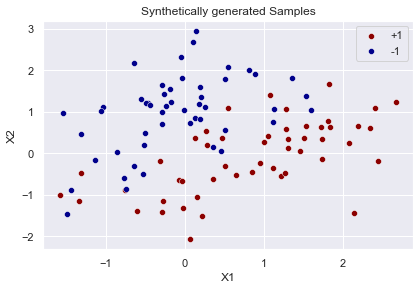
\includegraphics[width=\linewidth]{images/p1a/1/1.png}
        \end{column}
    \end{columns}

    \begin{columns}[]

        \begin{column}[]{0.30\linewidth}
            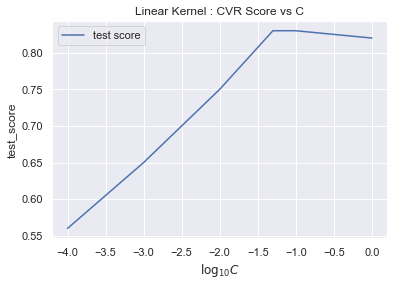
\includegraphics[width=\linewidth,height=90px]{images/p1a/1/l1.png}
            
             \centering $C_{opt} =1e^{-1}$
        \end{column}
        \begin{column}[]{0.40\linewidth}
            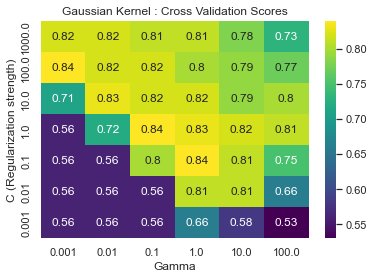
\includegraphics[width=\linewidth]{images/p1a/1/h1.png}
           

            \centering $C_{opt} = 1e^{0}$ 
            \centering $\gamma _{opt} = 1e^{-1}$
        \end{column}
        \begin{column}[]{0.40\linewidth}
            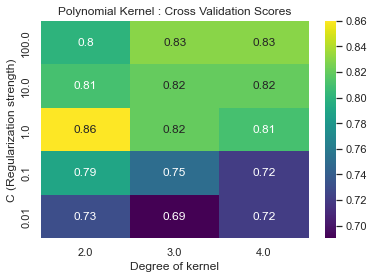
\includegraphics[width=\linewidth]{images/p1a/1/h2.png}
            \centering $degree_{opt} = 2$ 
            \centering $C_{opt} = 1e^{0}$
        \end{column}
    \end{columns}
\end{frame}

% VISUALIZATION OF CONTOURS Boundry
\begin{frame}[t]
    \scriptsize
    \large Surface boundry visualization 

    \begin{columns}
        \begin{column}[]{0.5\linewidth}
            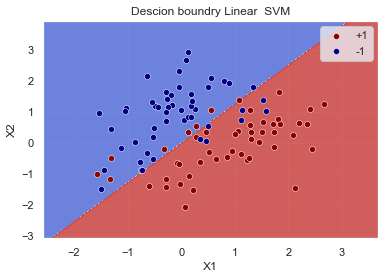
\includegraphics[width=\linewidth]{./images/p1a/1/d1.png}
        \end{column}
        \begin{column}[]{0.5\linewidth}
            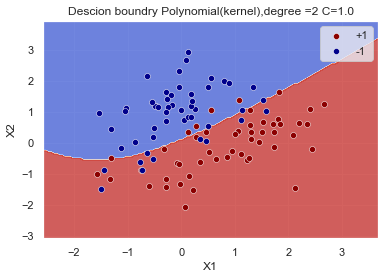
\includegraphics[width=\linewidth]{images/p1a/1/d2.png}
        \end{column}
        
    \end{columns}

    \begin{columns}
        \begin{column}[]{0.5\linewidth}
            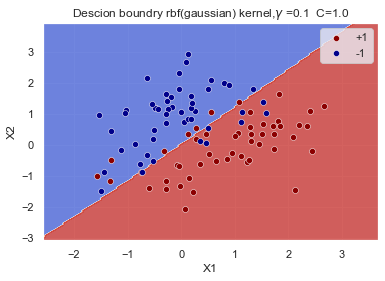
\includegraphics[width=\linewidth]{images/p1a/1/d3.png}
        \end{column}
        \begin{column}[]{0.5\linewidth}
            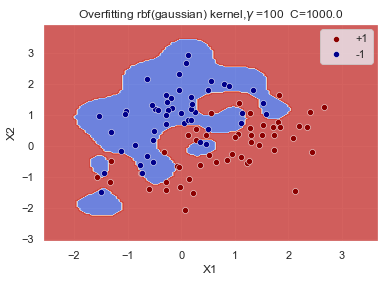
\includegraphics[width=\linewidth]{images/p1a/1/overfit1.png}
        \end{column}
        
    \end{columns}
\end{frame}

% Observations
\begin{frame}[t]
\scriptsize
\large Observation of the Synthetic 2d Data

\begin{enumerate}
    \scriptsize
    \item Higher values of \textbf{$\gamma$} cause the rbf kernel svm to \textbf{overfit}
    \item Best Hyperparameter Configuration are present in the \textbf{opposite diagonal}
            of the heatmap 
    \item C \textbf{regularization cofficient} : low value of C implies underfitting ,
            higher values of C cause overfitting
            
            $$ \min \frac{1}{2} ||w||^{2} + C \sum{\alpha_{i}}$$

            \centering High values of C cause w to dominate , hence the optimzed
            solution cause high w and hence low margin . For low value of C , we have
            opposite scenario
\end{enumerate}
\end{frame}


% BINARY CLASSIFICATION
\subsubsection{Binary Classification}

\begin{frame}[t]{Binary Classification}
    \scriptsize
    \begin{block}{Problem Statment}
        \begin{enumerate}
            \item Select Any two classes out of 10 , and create a binary classifier.
            \item \textbf{Chosen classes number 1 and 4}
            \item Try tuning the model with different Hyperparameter for various kernels.
            \item Interested Kernels are \textbf{gaussian(rbf), linear, polynomial}
        \end{enumerate}

        
    \end{block}
    \begin{block}{Hyperparameter tuning}
        \begin{enumerate}
            \item Using \textbf{GridSearchCV} class implemeted in \textbf{search.py}. (My own implementation)
            \item Since for each kernel there are \textbf{atmost 2 hyperparamters} thus using \textbf{HEATMAP} analysis 
                we get the best hyperparamters for our binary Classification problem
        \end{enumerate}
    \end{block}
\end{frame}

% Binary classification 10f -rbf kernel
\begin{frame}[t]{Binary Classification :(rbf)-10 features}
    \scriptsize

    \begin{columns}
        \begin{column}[T]{0.35\linewidth}
            On right is the \textbf{HeatMap} for cross validation scores , for Interested range
            of ($\gamma ,\mathcal{C}$). \\ 

            Calculated use \textbf{LIBSVM} python package.


            \begin{block}{Best hyperparamters}
                \begin{enumerate}
                    \item $\gamma = 0.1$ and  $\mathcal{C} = 1.0$ 
                    \item CV Score  $ = 0.9909318$
                \end{enumerate}
                    
            \end{block}

            \begin{block}{CV Score from SVM-CVXOPT}
                \begin{enumerate}
                    \item SVM-CVXOPT : SVM impl using convex opt package
                    \item CV Score $0.99094326$
                \end{enumerate}
            \end{block}
  
        \end{column}
        \begin{column}[T]{0.7\linewidth}
            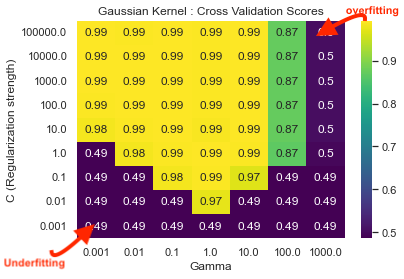
\includegraphics[width=\linewidth]{images/p1a/2(binary clf)/classes1and4_libsvm_rbf.png}
        \end{column}
    \end{columns}

\end{frame}

% Binary Classification -25f rbf kernel
\begin{frame}[t]{Binary Classification :(rbf)-25 features}
    \scriptsize

    \begin{columns}
        \begin{column}[T]{0.50\linewidth}
            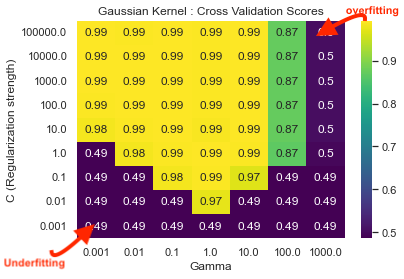
\includegraphics[width=\linewidth]{images/p1a/2(binary clf)/classes1and4_libsvm_rbf.png}
            \centering 10 features
        \end{column}
        \begin{column}[T]{0.50\linewidth}
            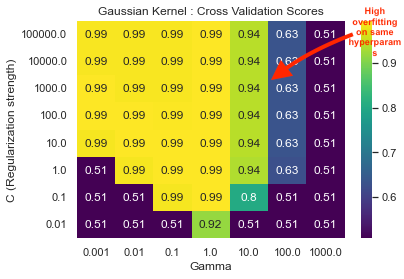
\includegraphics[width=\linewidth]{images/p1a/2(binary clf)/classes1and4_libsvm_rbf25f.png}
            \centering 25 features
        \end{column}
    \end{columns}

    \begin{block}{Observation}
        \begin{enumerate}
            \item Due to more number of features , \textbf{The model starts overfitting} soon 
                with high value of $\gamma$ and C.
            \item Look for $\gamma =100$
        \end{enumerate}
    \end{block}
\end{frame}

% Binary Classification 10f  Linear Kernel : 

\begin{frame}[t]{Binary Classification :(linear) -10 features}
    \scriptsize

    \begin{columns}
        \begin{column}[T]{0.35\linewidth}
            On right is the \textbf{PLOT} for cross validation scores , for Interested range
            of ($\mathcal{C}$). \\ 

            Calculated use \textbf{LIBSVM} python package.


            \begin{block}{Best hyperparamters}
                \begin{enumerate}
                    \item  $\mathcal{C} = 1.0$ 
                    \item CV Score  $ = 0.9909318$
                \end{enumerate}
                    
            \end{block}

            \begin{block}{CV Score from SVM-CVXOPT}
                \begin{enumerate}
                    \item SVM-CVXOPT : SVM impl using convex opt package
                    \item CV Score $0.99092048$
                \end{enumerate}
            \end{block}
  
        \end{column}
        \begin{column}[T]{0.7\linewidth}
            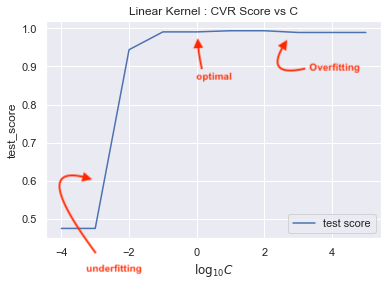
\includegraphics[width=\linewidth]{images/p1a/2(binary clf)/classes1and4_libsvm_linear10f.png}
        \end{column}
    \end{columns}
\end{frame}

% Binary Classification -25f linear kernel
\begin{frame}[t]{Binary Classification :(linear)-25 features}
    \scriptsize

    \begin{columns}
        \begin{column}[T]{0.50\linewidth}
            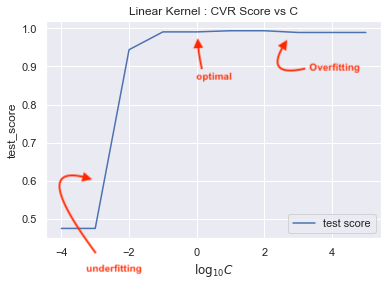
\includegraphics[width=\linewidth]{images/p1a/2(binary clf)/classes1and4_libsvm_linear10f.png}
            \centering 10 features
        \end{column}
        \begin{column}[T]{0.50\linewidth}
            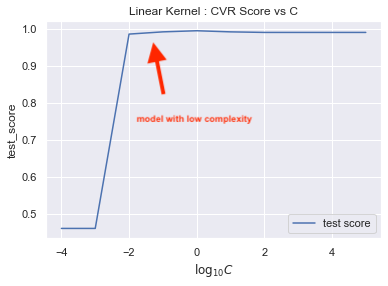
\includegraphics[width=\linewidth]{images/p1a/2(binary clf)/classes1and4_libsvm_linear25f.png}
            \centering 25 features
        \end{column}
    \end{columns}

    \begin{block}{Observation}
        \begin{enumerate}
            \item Due to more number of features , \textbf{The model starts overfitting} soon 
                with high value of $\gamma$ and C.
            \item Thus C=1 worked 10 feature case , not C=0.1 works the same for 25 features.
        \end{enumerate}
    \end{block}
\end{frame}

% Binary Classification-10f (polynomial)

\begin{frame}[t]{Binary Classification :(polynomial) -10 features}
    \scriptsize

    \begin{columns}
        \begin{column}[T]{0.35\linewidth}
            On right is the \textbf{PLOT} for cross validation scores , for Interested range
            of ($ degree, \mathcal{C}$). \\ 

            Calculated use \textbf{LIBSVM} python package.


            \begin{block}{Best hyperparamters}
                \begin{enumerate}
                    \item  $\mathcal{C} = 10$
                    \item $degree = 3$ 
                    \item CV Score  $ = 0.99244$
                \end{enumerate}
                    
            \end{block}

            \begin{block}{CV Score from SVM-CVXOPT}
                \begin{enumerate}
                    \item SVM-CVXOPT : SVM impl using convex opt package
                    \item CV Score $0.9924584$
                \end{enumerate}
            \end{block}
  
        \end{column}
        \begin{column}[T]{0.7\linewidth}
            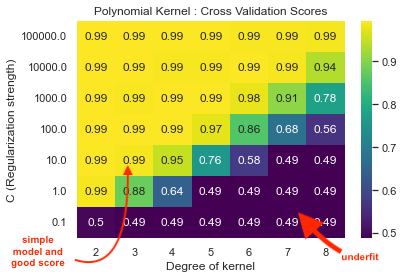
\includegraphics[width=\linewidth]{images/p1a/2(binary clf)/classes1and4_libsvm_poly10f.png}
        \end{column}
    \end{columns}
\end{frame}

% Binary Classification -25f polynomial kernel
\begin{frame}[t]{Binary Classification :(polynomial)-25 features}
    \scriptsize

    \begin{columns}
        \begin{column}[T]{0.50\linewidth}
            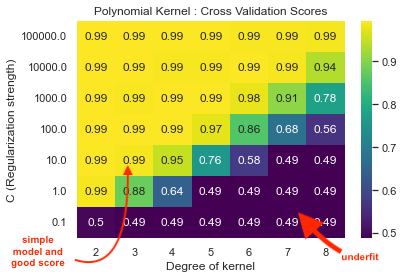
\includegraphics[width=\linewidth]{images/p1a/2(binary clf)/classes1and4_libsvm_poly10f.png}
            \centering 10 features
        \end{column}
        \begin{column}[T]{0.50\linewidth}
            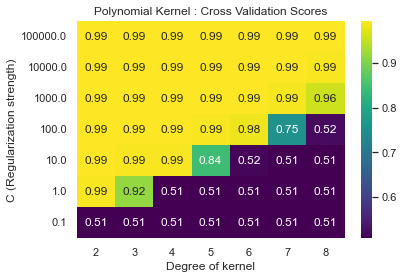
\includegraphics[width=\linewidth]{images/p1a/2(binary clf)/classes1and4_libsvm_poly25f.png}
            \centering 25 features
        \end{column}
    \end{columns}

    \begin{block}{Observation}
        \begin{enumerate}
            \item Configurations where \textbf{polynomial kernel} had underfitting with 10 features , some 
                of them  now have a good fit with increased number of features i.e 25.
            \item There is \textbf{No overfitting }in polynomial kernel with given data set
            \item Increase in feature cause shift of underfit along the primary diagonal of the HEATMAP
        \end{enumerate}
    \end{block}
\end{frame}


% Binary Classification :(linear)More Pair of classes
\begin{frame}[t]{Binary Classification:(linear) More pair of classes}
\scriptsize
\begin{columns}
    \begin{column}[]{0.25\linewidth}
        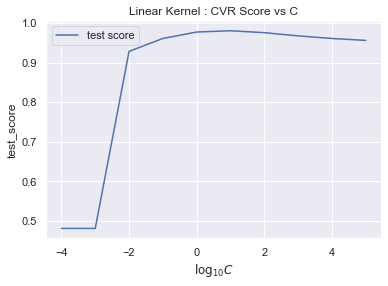
\includegraphics[width=\linewidth]{images/p1a/2(binary clf)/classes2and7_libsvm_linear25f.png}
        \centering classes 2,7
    \end{column}
    \begin{column}[]{0.25\linewidth}
        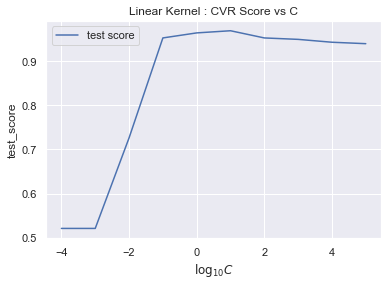
\includegraphics[width=\linewidth]{images/p1a/2(binary clf)/classes3and9_libsvm_linear25f.png}
        \centering classes 3,9
    \end{column}
    \begin{column}[]{0.25\linewidth}
        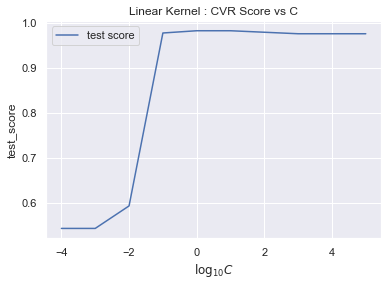
\includegraphics[width=\linewidth]{images/p1a/2(binary clf)/classes4and8_libsvm_linear25f.png}
        \centering classes 4,8
    \end{column}
    \begin{column}[]{0.25\linewidth}
        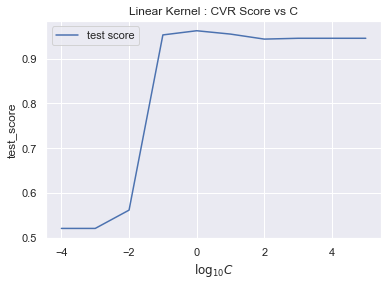
\includegraphics[width=\linewidth]{images/p1a/2(binary clf)/classes5and6_libsvm_linear25f.png}
        \centering classes 5,6
    \end{column}
    
\end{columns}

\begin{columns}
    \begin{column}[]{0.25\linewidth}
        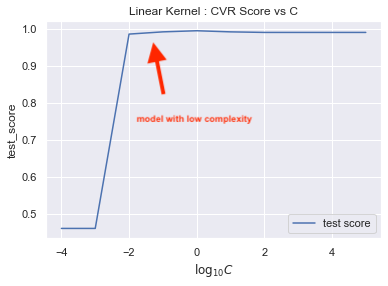
\includegraphics[width=\linewidth]{images/p1a/2(binary clf)/classes1and4_libsvm_linear25f.png}
        classes 1,4
    \end{column}
    \begin{column}[]{0.75\linewidth}
        \begin{block}{Observation}
            \begin{enumerate}
                \item \textbf{Same Hyperparameter i.e C=0.1} works for all above pair of classes
                \item \textbf{Got consistently Best result} with same hyperparamters.
            \end{enumerate}
        \end{block}
    \end{column}
\end{columns}
    

\end{frame}

% Binary Classification :(gaussian) More Pair of classes
\begin{frame}[t]{Binary Classification:(gaussian) More pair of classes}
    \scriptsize
    \begin{columns}
        \begin{column}[]{0.33\linewidth}
            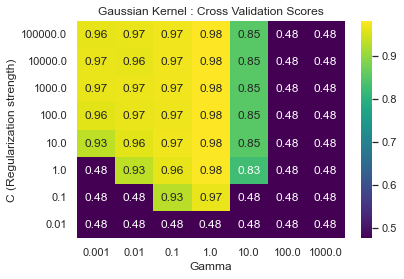
\includegraphics[width=\linewidth]{images/p1a/2(binary clf)/classes3and9_libsvm_rbf25f.png}
            \centering classes 3,9
        \end{column}
        \begin{column}[]{0.33\linewidth}
            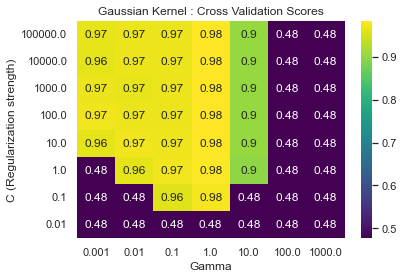
\includegraphics[width=\linewidth]{images/p1a/2(binary clf)/classes2and4_libsvm_rbf25f.png}
            \centering classes 2,4
        \end{column}
        \begin{column}[]{0.33\linewidth}
            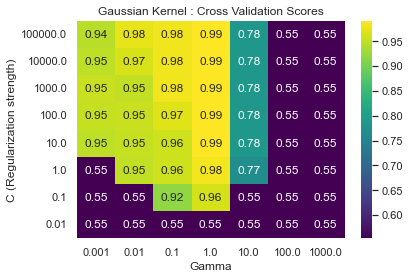
\includegraphics[width=\linewidth]{images/p1a/2(binary clf)/classes2and5_libsvm_rbf25f.png}
            \centering classes 2,5
        \end{column}
    \end{columns}
    
    \vspace{10pt}

    \begin{columns}
        \begin{column}[T]{0.33\linewidth}
            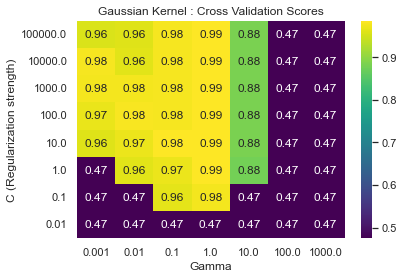
\includegraphics[width=\linewidth]{images/p1a/2(binary clf)/classes6and8_libsvm_rbf25f.png}
            \centering classes 6,8
        \end{column}
        \begin{column}[T]{0.66\linewidth}
            \begin{block}{Observation}
                \begin{enumerate}
                    
                    \item \textbf{Got consistently Best result} with same hyperparamters, evem with gaussian kernel
                 
                    \item $\gamma =0.1 , C=1$
                \end{enumerate}
            \end{block}
        \end{column}
    \end{columns}
        
\end{frame}


%% Multiclass Classification

\subsubsection{Multi Class Classification}
\begin{frame}
    \frametitle{Multi-Class Classification}
    \scriptsize
    \begin{block}{Problem Statment}
        \begin{enumerate}
            \item Using LIBSVM implemeted in SVMLIBSVM.py
            \item Try tuning the model with different Hyperparameter for various kernels.
            \item Interested Kernels are \textbf{gaussian(rbf), linear, polynomial}
        \end{enumerate}

        
    \end{block}
    \begin{block}{Hyperparameter tuning}
        \begin{enumerate}
            \item Using \textbf{GridSearchCV} class implemeted in \textbf{search.py}. (My own implementation)
            \item Since for each kernel there are \textbf{atmost 2 hyperparamters} thus using \textbf{HEATMAP} analysis 
                we get the best hyperparamters for our binary Classification problem
        \end{enumerate}
    \end{block}
    

\end{frame}

% Multiclass clf :(linear)
\begin{frame}[t]{Multilclass Classification :(linear)}

    \scriptsize

    \begin{columns}
        \begin{column}[T]{0.5\linewidth}
            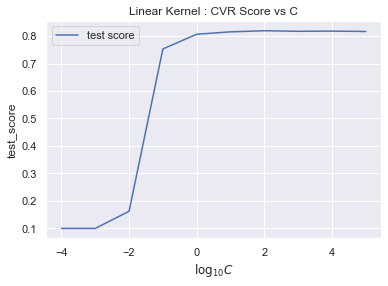
\includegraphics[width=\linewidth,height=80pt]{images/p1a/3(multiclass)/multilibsvm_linear10f.png}
            \vspace{-2pt}
            \centering Feature =10 , best cv-score (0.8193)

            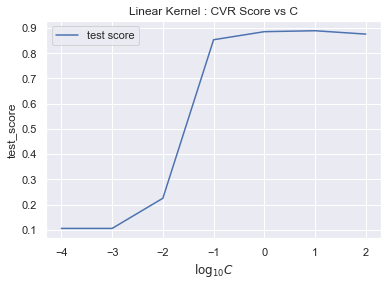
\includegraphics[width=\linewidth,height=80pt]{images/p1a/3(multiclass)/multilibsvm_linear25f.png}
            \vspace{-2pt}
            \centering Feature =25 , best cv-score (0.889)


        \end{column}
        \begin{column}[T]{0.5\linewidth}
            \begin{block}{Observation}
                \begin{enumerate}
                    \item \textbf{Best hyperparamters remains same} as they were in case of binary clf.
                    \item The \textbf{best cv-score(0.8193)} in 10-feature case and \textbf{0.889} in 25-features case , is less as compared to binary clf(around \textbf{0.99})
                    \item \textbf{More number of features}(25 feature case) \textbf{generalizes} the multiclass desicion boundry.
                \end{enumerate}
            \end{block}
        \end{column}        
    \end{columns}


\end{frame}

% Multiclass clf :(rbf)
\begin{frame}[t]{Multilclass Classification :(rbf)}

    \scriptsize

    \begin{columns}
        \begin{column}[T]{0.5\linewidth}
            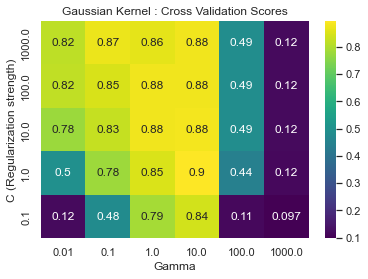
\includegraphics[width=\linewidth,height=80pt]{images/p1a/3(multiclass)/multilibsvm_rbf10f.png}
            \vspace{-2pt}
            \centering Feature =10 , best cv-score (0.8953)

            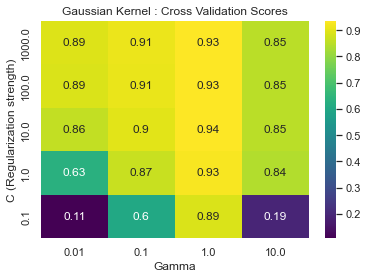
\includegraphics[width=\linewidth,height=80pt]{images/p1a/3(multiclass)/multilibsvm_rbf25f.png}
            \vspace{-2pt}
            \centering Feature =25 , best cv-score (0.9445)


        \end{column}
        \begin{column}[T]{0.5\linewidth}
            \begin{block}{Observation}
                \begin{enumerate}
                    \item \textbf{Best hyperparamters remains same} as they were in case of binary clf.
                    \item The \textbf{best cv-score(0.8952)} in 10-feature case and \textbf{0.9445} in 25-features case , is less as compared to binary clf(around \textbf{0.99})
                    \item \textbf{More number of features}(25 feature case) \textbf{generalizes} the multiclass desicion boundry.
                \end{enumerate}
            \end{block}


            \begin{block}{Notice}
                \begin{itemize}
                    \item Training time of the SVM model is very highly sensitive to values of C .
                         thus while performing 
                        GridSearch for 25 feature case , a smaller Hyperparameter space is used.
                \end{itemize}
            \end{block}
        \end{column}        
    \end{columns}


\end{frame}

\begin{frame}
    \frametitle{Multiclass classification :Conclusion}
    \scriptsize
    \begin{enumerate}
        \item Best score of 0.9445 with kernel 'rbf' which is quite less compared to binary Classification

    \end{enumerate}
    \begin{block}{One vs One Classification -LIBSVM}
        \begin{enumerate}
            \item One-vs-One  is another heuristic method for using binary 
            classification algorithms for multi-class classification.
            \item one-vs-one splits a multi-class classification dataset
            into binary classification problems
            \item There are $n(n-1)/2$ models trained 
            \item Each binary classification model may predict one class label and the model 
            with the most predictions or votes is predicted by the one-vs-one strategy.
        \end{enumerate}
    

        
    \end{block}

    

\end{frame}


\subsection{Part- 1B}
\begin{frame}
    \frametitle{SMO}

    \begin{block}{SMO general algorithm}
        \begin{enumerate}
            \item Find a Lagrange multiplier $\alpha_{1}$ that violates the Karush–Kuhn–Tucker (KKT) conditions for the optimization problem.
            \item Pick a second multiplier $\alpha_{2}$ and optimize the pair $(\alpha_{1},\alpha_{2})$.
            \item Repeat steps 1 and 2 until convergence.
        \end{enumerate}
    \end{block}

    \begin{block}{Note}
        Although this algorithm is guaranteed to converge, heuristics are used to choose
         the pair of multipliers so as to accelerate the rate of convergence.
         This is critical for large data sets since there are 
         $\frac{n(n-1)}{2}$ possible choices for $\alpha_{i}$ and 
         $\alpha_{j}$.
    \end{block}
    

\end{frame}
\begin{frame}
    \frametitle{Simplified SMO}
    \scriptsize
    Implemented from CS229 lecture notes.

    \large Training SVM on non-linear case 
    \begin{columns}[]
        \begin{column}[]{0.5\linewidth}
            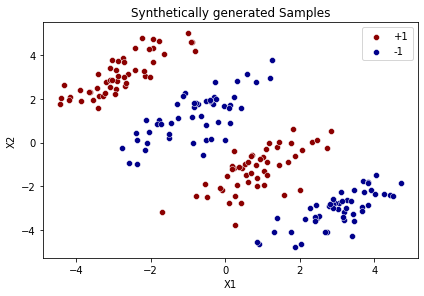
\includegraphics[width=\linewidth]{images/p1c/data.png}
        \end{column}
        \begin{column}[]{0.5\linewidth}
            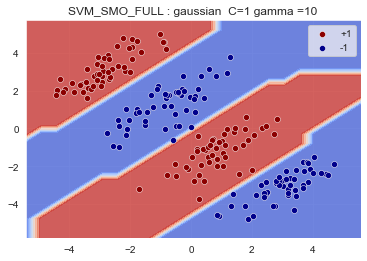
\includegraphics[width=\linewidth]{images/p1c/simplesmo_rbf.png}
        \end{column}

    \end{columns}

    \scriptsize
    \begin{block}{Observation}
        \begin{enumerate}
            \item Since the simplified SMO uses random heuristics while choosing pairs of alpha 
                thus theoritically we cannot proove convergence of this Algorithm.
            \item Simplified SMO is faster than CVXOPT .
        \end{enumerate}
    \end{block}
    
    
\end{frame}
\subsection{Part- 1C}
\begin{frame}
    \frametitle{SMO Complete- Choosing heuristics}
    \scriptsize
    \centering \textbf{First Choice heuristics}
    
    \begin{enumerate}
        \item As the SMO algorithm progresses, examples that are at the bounds are
         likely to stay at the bounds, while examples that are not at the bounds will
          move as other examples are optimized.
        \item  First langrange multiplier is chosen out of unbounded examples
    \end{enumerate}

    \centering \textbf{Second choice heuristics}

   
    \begin{enumerate}
        \item Once a first Lagrange multiplier is chosen, SMO chooses the second Lagrange multiplier
                 to maximize the size of the step taken during joint optimization
        \item SMO keeps a cached error value E for every non-bound point in the training 
        set and then chooses an error to approximately maximize the step size
        \item  If E1 is positive, SMO chooses an point with minimum error E2. 
            If E1 is negative, SMO chooses an point with maximum error E2.
        \item if SMO cannot make positive progress using the second choice heuristic
        \begin{enumerate}
            \scriptsize
            \item  then SMO starts iterating through the non-bound examples, searching for an second example that can make positive progress
            \item If none of the non-bound examples make positive progress, then SMO starts iterating through the entire training set until
             an example is found that makes positive progress
             \item In extremely degenerate circumstances, none of the examples will make an adequate second example. We skip the first langrange multiplier
        \end{enumerate}
    \end{enumerate}
    

\end{frame}

\begin{frame}
    \scriptsize
    \frametitle{SMO Complete}
    The code for SMO was implemeted Using the pseudo code in John platt paper .
    The class is implemeted in SVM\_SMO\_FULL.py
    \\

    \cite[Sequential Minimal Optimization:
    A Fast Algorithm for Training Support Vector Machines , John Platt]{}

    \large Training SVM on non-linear case 

    \begin{columns}[]
        \begin{column}[]{0.34\linewidth}
            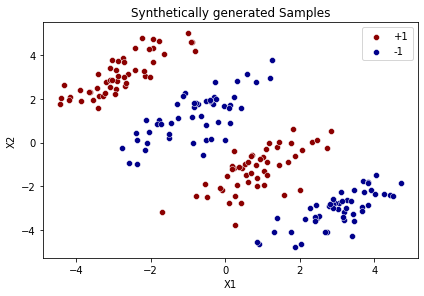
\includegraphics[width=\linewidth]{images/p1c/data.png}
        \end{column}
        \begin{column}[]{0.34\linewidth}
            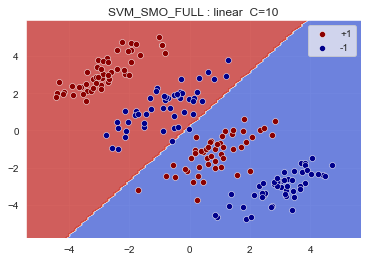
\includegraphics[width=\linewidth]{images/p1c/linear_results.png}
        \end{column}
        \begin{column}[]{0.34\linewidth}
            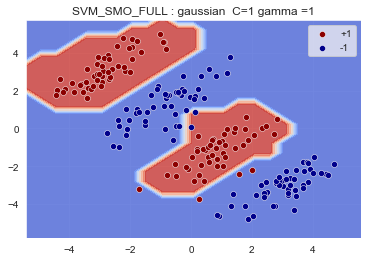
\includegraphics[width=\linewidth]{images/p1c/gausian_results.png}
        \end{column}
    \end{columns}

    \scriptsize
    \begin{block}{Observation}
        \begin{enumerate}
            \item My implementation of SMO was faster than SVM\_CVX , but slower in run time than standard
            LIBSVM  
        \end{enumerate}
    \end{block}

\end{frame}

\section{Part-2}

\begin{frame}[t]
    \frametitle{Part-2 Classification Problem}
    \scriptsize
    This part of the problem has been solved in  the P2.ipynb .
    \begin{enumerate}
        \item Used \textbf{HeatMap visualization on GridSearchCV} results to tune the hyperparamters.
        \item \textbf{kernel : gaussian dominated} after training few models , so I have fine tuned the 
            paramters C and $\gamma$ in the gaussian kernel
    \end{enumerate}

    \begin{columns}[]
        \begin{column}[]{0.25\linewidth}
            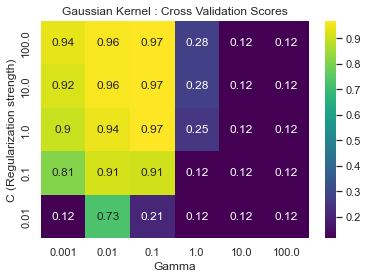
\includegraphics[width=\linewidth,height=70pt]{images/p2/1.png}
        \end{column}
        \begin{column}[]{0.25\linewidth}
            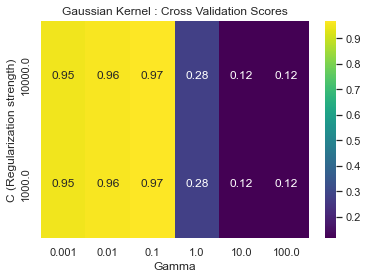
\includegraphics[width=\linewidth,height=70pt]{images/p2/2.png}
        \end{column}
        \begin{column}[]{0.25\linewidth}
            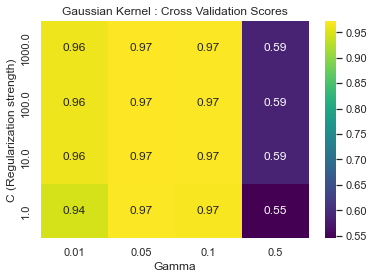
\includegraphics[width=\linewidth,height=70pt]{images/p2/3.png}
        \end{column}
        \begin{column}[]{0.25\linewidth}
            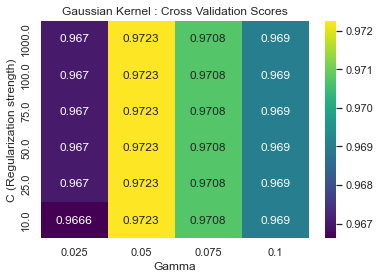
\includegraphics[width=\linewidth,height=70pt]{images/p2/5.png}
        \end{column}
    \end{columns}

    \begin{block}{Best Hyperparamters}
        \begin{enumerate}
            \item $C= 10$
            \item $\gamma =0.05$
            \item kernel : gaussian/rbf
            \item  Score on Kaggle submission $=0.96875$
        \end{enumerate}
    \end{block}
    

\end{frame}
\end{document}